\subsection{40}
\begin{myfrag}
Was ist die kanonische Zustandssumme? Leite den Erwartungswert der Energie
als Ausdruck der Zustandssumme her.
\end{myfrag} \quad \\
Kanonische Zustandsumme: \\
$ Z= \sum \limits_r \exp ^{-\beta \epsilon _r} $ \quad \\ Zustandsintegral  $Z = \int d \Gamma \exp ^{-\beta H} $ \\[1ex]
Erwartungswert:$ \left\langle A_r \right\rangle = \dfrac{\sum _r \exp ^{-\beta \epsilon _r}}{Z}$ \\[1ex]
$\Rightarrow \left\langle E \right\rangle = \dfrac{\sum _r \epsilon _r \exp ^{-\beta \epsilon _r}}{Z} = \dfrac{\sum _r \dfrac{\partial}{\partial \beta} \exp ^{-\beta \epsilon _r}}{Z} = -\dfrac{\dfrac{\partial Z}{\partial \beta}}{Z} = - \dfrac{\partial lnZ}{\partial \beta}$
\subsection{41}
\begin{myfrag}
Wie ist die Freie Energie definiert? Wie können Energie, Entropie sowie
generalisierte Kräfte (Druck, etc.) als Funktion der Freien Energie berechnet
werden?
\end{myfrag} \quad \\
Freie Energie : $ F = -k_B T lnZ \\[1ex]
E = \dfrac{\partial (\beta F)}{\partial \beta } = - \dfrac{\partial lnZ}{\partial \beta } \\[1ex]
S= - \left( \dfrac{\partial F}{\partial T} \right) _\alpha = k_BlnZ + \dfrac{E}{T} \\[1ex]
F_\alpha =- \left( \dfrac{\partial E}{\partial \alpha } \right)_S = - \left( \dfrac{\partial F}{\partial \alpha } \right) _T \qquad p = - \left( \dfrac{\partial F}{\partial V} \right)_T \qquad m= - \left( \dfrac{\partial F}{\partial B} \right)_T$ 
\subsection{42}
\begin{myfrag}
Vergleiche die Konzepte des Kanonischen und des Mikrokanonischen Ensembles
in einer Liste: Was ist die jeweilige physikalische Situation? Was ist jeweils die
Zustandssumme und das zentrale thermodynamische Potential? Wie werden
thermodynamische Größen (gen. Kräfte, Druck, Temperatur, Energie und
Entropie) bestimmt? Was sind die Besetzungswahrscheinlichkeiten?
\end{myfrag} \quad \\
$\begin{array}{l | l}
$Mikrokan. Ensemble$ & $Kanonisches Ensemble$ \\ \hline 
$Annahme: isoliert, E = const $ & $ in thermischen Kontakt, T = const $ 
\\[1.5ex]
$Zustandsintegral $ \Omega = \int d \Gamma \delta (E-H(\{\vec{r} _i , \vec{p} _i \} )) & $ Zustandsintegral $ Z= \int d \Gamma \exp ^{-\beta H(\{ \vec{r} _i , \vec{p} _i \} ) } 
\\[1.5ex]
 $zentrales Thermodyn. Potential $ S=k:Bln \Omega & F=-k_B T ln Z 
\\
P_r = \dfrac{1}{\Omega} 
&
 P_r = \dfrac{\exp^{-\beta \epsilon _r}}{Z}
 \\[1.5ex]
\dfrac{1}{T}= \left( \dfrac{\partial S}{\partial E} \right) _{V,N} 
& 
E= - \dfrac{\partial lnZ}{\partial \beta} = \dfrac{\partial (\beta F)}{\partial
 \beta} 
\\[1.5ex]
F_\alpha = T\left( \dfrac{\partial S}{\partial \alpha } \right) _{E} & F_\alpha = - \left( \dfrac{\partial S}{\partial \alpha } \right) _{T}
\end{array} $
\subsection{43}
\begin{myfrag}
Wende die Methoden des Kanonischen Ensembles auf das Ideale Klassische Gas
an. Rechne die Erwartungswerte für den Druck, die Energie und die Entropie aus.
\end{myfrag} \quad \\
klassisches ideales Gas: \\
$Z = \int \prod \limits _{i=1}^N d^3 \vec{r} _i \prod \limits_{i=1}^N d^3 \vec{p} _i \exp ^{-\beta \sum \limits_i \dfrac{p_i^2}{2m} } \qquad $NR: $ \int dp_x dp_y dp_y \exp ^{-\beta \dfrac{p_x^2+p_y^2+p_z^2}{2m}}=(\int dy \exp ^{\alpha y^2})^3  
\\
 = V^N\left( \sqrt{\dfrac{2m \pi}{\beta}} \right) ^{3N} = V^N(2m\pi k_B T)^{\dfrac{3N}{2}} \qquad \qquad \qquad \qquad = \left( \sqrt{ \dfrac{ \pi }{\alpha }}\right) ^2
 \\
 F= -k_B TlnZ = -k_B T N (lnV + \dfrac{2}{3}lnT + const) 
 \\[1ex]
E= - \dfrac{\partial lnZ}{\partial \beta} = \dfrac{\partial N(lnV - \dfrac{2}{3}lnT + const}{\partial \beta} = \dfrac{3N}{2\beta}= \dfrac{3}{2} Nk_B T
\\[1ex]
p= -\left(\dfrac{\partial F}{\partial V} \right) _T = k_B TN \dfrac{\partial lnV}{\partial V} = \dfrac{k_B TN}{V} \quad \Rightarrow \quad pV= Nk_B T
\\[1ex]
S= \dfrac{E_F}{T} = k_BlnZ + \dfrac{E}{T} =k_B N (lnV + \dfrac{3}{2}lnT+ const)+\dfrac{3}{2} N k_B$
\subsection{44}
\begin{myfrag}
Betrachte ein vereinfachtes quantisiertes Modell für ein „Polymer“, wobei die
einzelnen Polymerglieder der Länge d nur nach links oder rechts zeigen können.
Berechne den Erwartungswert der Länge L mit Hilfe des Kanonischen Ensembles
als Funktion der Kraft (siehe auch Frage 37.).
\end{myfrag} \quad \\
$Z= \sum \limits_{Zustaende} \exp ^{-\beta H}
= \sum \limits_{r_j=\pm} \exp ^{-\beta \sum \limits_j H_j} \qquad j = 1,...,N  \quad r_j = \pm $ Zustand des Segments j$
\\[1.5ex]
H= \sum \limits_j H_j \qquad H_j = r_j Fd= \pm Fd 
\\[1.5ex]
Z = \sum \limits _{r_j = \pm } \exp ^{-\beta \sum \limits _j H_j}= \prod \limits_{j=1}^N \sum \limits _{r=\pm} \exp ^{-\beta rFd}
\\[1.5ex]
Z_1 = \sum \limits_{r=\pm} \exp ^{-\beta rFd} = \exp ^{-\beta Fd} = \exp ^{-\beta Fd} + \exp ^{\beta Fd} = 2cosh(\beta Fd)
\\[1.5ex]
L=N\left\langle l \right\rangle \qquad l=rd=\pm d \qquad \left\langle l \right\rangle = \dfrac{\sum \limits _{r=\pm} \exp ^{-\beta rFd} rd}{Z_1}
\\[1.5ex]
P_r = \dfrac{\exp ^{-\beta H_1(r)}}{Z_1} \qquad \left\langle A \right\rangle = \sum \limits _r P_r A_r = \dfrac{\sum \limits _r A_r \exp ^{-\beta H(r)}}{Z} 
\\[1.5ex]
\left\langle l \right\rangle = \dfrac{d\exp ^{-\beta Fd} -d\exp ^{\beta Fd}}{cosh(\beta Fd)} = -d \dfrac{sinh(\beta Fd)}{cosh(\beta Fd)} \qquad L= \left\langle l \right\rangle = Ndtanh(\beta Fd) 
\\[1.5ex]
$Umkehrung : $F=\dfrac{k_BT}{2d}ln\left( \dfrac{Nd-L}{Nd+L} \right) $ im Mikrokanonischen Ensemble.

\subsection{45}
\begin{myfrag}
Berechne die Mischentropie für zwei ideale Gase. Erläutere ausführlich das
Gibbssche Paradoxon und dessen Lösung.
\end{myfrag} \quad \\

\begin{minipage}[l]{0.3\textwidth}
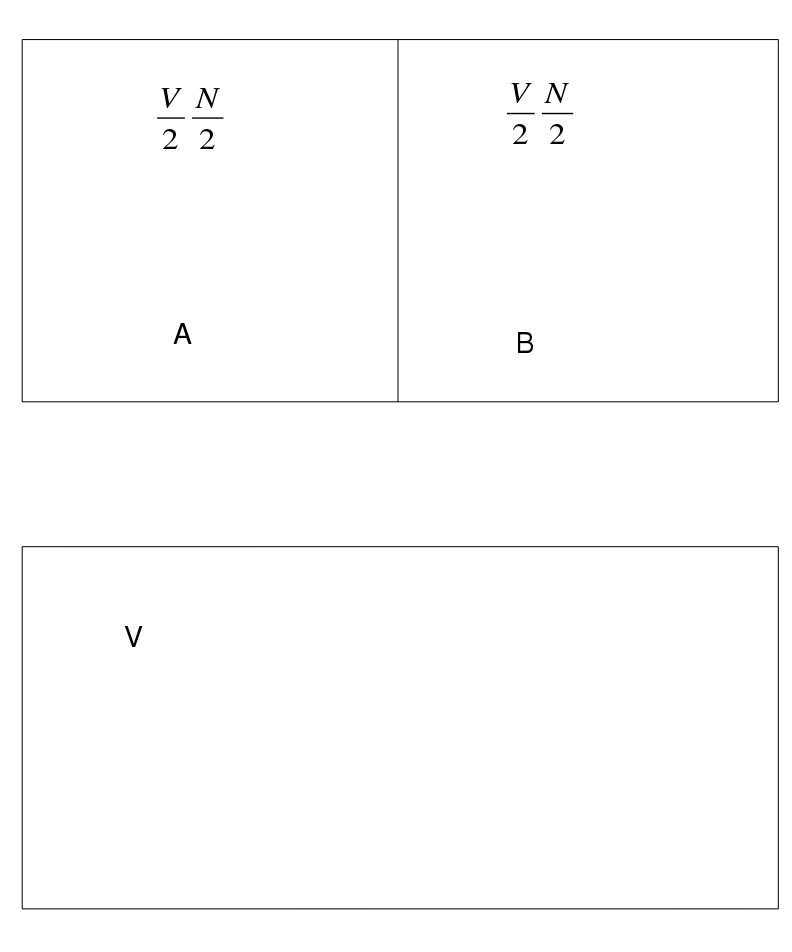
\includegraphics[width=4.2cm]{Bilder/Frage45eins.jpg} 
\end{minipage} 
\begin{minipage}[c]{0.69\textwidth}
$ S_{vorher} = S_1 + S_2
\\ 
= k_B \dfrac{N}{2} (ln \dfrac{V}{2} + \dfrac{3}{2}lnT + const) + k_B\dfrac{N}{2}(ln\dfrac{V}{2} + \dfrac{3}{2}lnT +const) 
\\
=k_BN(ln\dfrac{V}{2}+\dfrac{3}{2}lnT+const)$ \\[2ex]
$S_{nachher} = S_1+S_2
\\
=k_B\dfrac{N}{2}(lnV+\dfrac{3}{2}lnT +const) + k_B \dfrac{N}{2} (lnV + \dfrac{3}{2} lnT +const)
\\
= k_B N (lnV + \dfrac{3}{2} lnT + const)
\\
= S_{vor} + k_B Nln2$

\end{minipage}
\\[2ex]
Gibbsches Paradoxon: Für ununterscheidbare Gase gilt die gleiche Rechnung, aber der Prozess ist reversibel. \\[2ex]
\begin{minipage}[c]{0.3\textwidth}
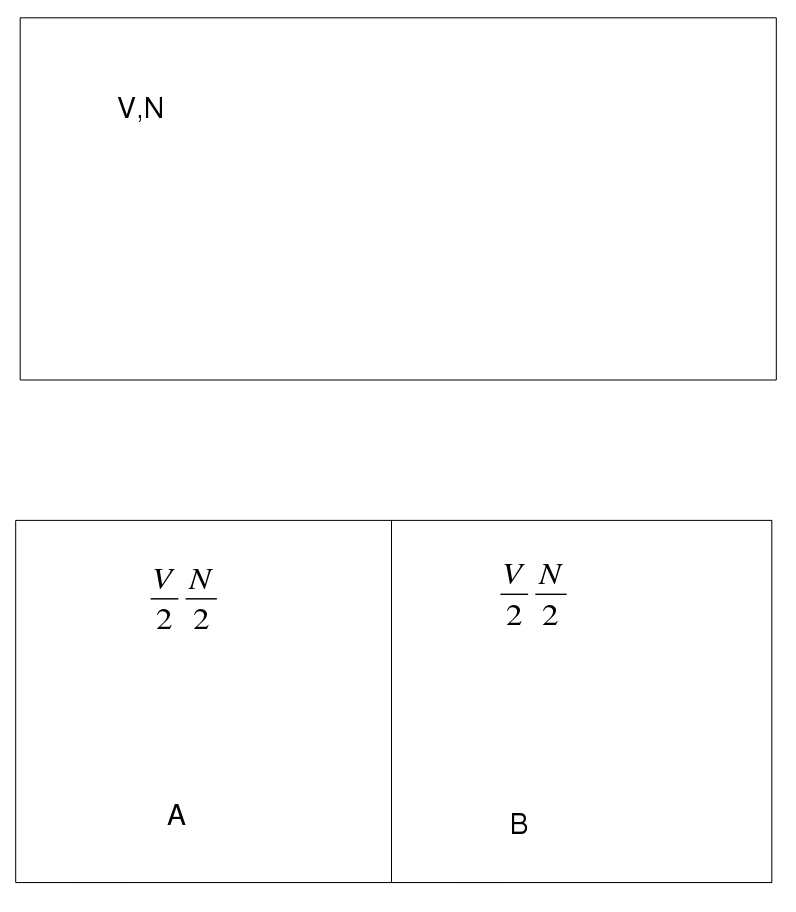
\includegraphics[width=4.2cm]{Bilder/Frage45zwei.jpg} 

\end{minipage}
\begin{minipage}[c]{0.69\textwidth}
$ S_{vorher} = k_B N(lnV + \dfrac{3}{2} lnT + const )
\\[9ex]
S_{nachher} = S_1 + S_2 
\\
= k_B \dfrac{N}{2} (ln\dfrac{V}{2} + \dfrac{3}{2} lnT + const ) + k_B \dfrac{N}{2}(ln\dfrac{V}{2} +\dfrac{3}{2} lnT +const)
\\
= k_B N (ln \dfrac{V}{2} + \dfrac{3}{2} lnT +const)
\\
= S_{vor} - k_B ln2 < S_{vor}$
\end{minipage}
\\[2ex]
Großer Unterschied ob Teilchen unterscheidbar oder nicht sollte reversibel sein, doch zählt Z zu viele Zustände. Also Zustandsumme für ununterscheidbarer Teilchen falsch berechnet \\[1.5ex]
$Z = \dfrac{1}{N!} \int d\Gamma \exp ^{- \beta H (\{\vec{r}_i,\vec{p}_i\})}$ \\[1.5ex]
Für unterscheidbaren Teilchensatz \\[1.5ex]
$Z=\dfrac{1}{N_a !} \dfrac{1}{N_b !}\dfrac{1}{N_c !}...\int d\Gamma \exp ^{- \beta H}$
\subsection{46}
\begin{myfrag}
Wann sind zwei Teilsysteme unabhängig? Was passiert mit der Zustandssumme,
den Wahrscheinlichkeiten und den Erwartungswerten in diesem Fall? Was
versteht man unter einer Einteilchenzustandssumme?
\end{myfrag} \quad \\
Falls Energien von Freiheitsgraden einfach addiert werden können, so sind diese \glqq unabhängig"
\\[1.5ex]
$ H (\{\vec{r}_i,\vec{p}_i\})= H_1 (\vec{r}_1,\vec{p}_1) + H_1 (\vec{r}_2,\vec{p}_2)+ ... = \sum \limits_{j=1}^N H_1( \vec{r}_j, \vec{p}_j)
\\[1.5ex]$
Z.B ideales Gas $ H_1 = \dfrac{p^2}{2m}$ \glqq Einteilchen Hamilton Operator" d.h. $V(\vec{r}_i - \vec{r} _j) = 0$ ( keine Wechselwirkung) 
\\[1.5ex]
$\Rightarrow Z_1 = \sum \limits _r \exp ^{-\beta H_1(r)}$ heißt Einteilchenzustandssumme (hängt nur von der Quantenzahl bzw. koordinaten eines Teilchens ab) 
\\[1.5ex]
$Z= \sum \limits _{\{r_j\}} \exp ^{-\beta \sum \limits_j H(r_j)} = \left\lbrace \begin{array}{c c}
Z_1^N &  $bei unterscheidbaren Teilchen$ 
\\[1.5ex]
\dfrac{Z_1^N}{N!} & $ bei unterscheidbaren Teilchen $
\end{array} \right.$
\\[1.5ex]
Wahrscheinlichkeiten: \\[1.5ex]
$H= H_A(r_A) +H_B(r_B) 
\\[1.5ex]
P(r_A,r_B)=\dfrac{\exp ^{-\beta (H_A(r_A) + H_B(r_B))}}{\sum \limits _{r_A,r_B} \exp ^{-\beta (H_A(r_A) + H_B(r_B))}} = \dfrac{\exp ^{-\beta H_A(r_A)}}{\sum \limits _{r_A} \exp ^{-\beta H_A(r_A)}}\dfrac{\exp ^{-\beta H_B(r_B)}}{\sum \limits _{r_B} \exp ^{-\beta  H_B(r_B)}} = P_A(r_A)P_B(r_B)$ \\[1.5ex]
unabhängige Wahrscheinlichkeit
\subsection{47}
\begin{myfrag}
Argumentiere, dass die Änderung des statistischen Erwartungswertes der Energie
in Erwartungswerte für die Änderung von Wärme und Arbeit aufgeteilt werden
kann. Leite einen Zusammenhang mit Änderungen der Entropie und der
generalisierten Kräfte her.
\end{myfrag} \quad \\
$\left\langle E \right\rangle = \sum \limits _r P_r \epsilon _r \\[1.5ex]
dE = \sum \limits_r \epsilon _r dP_r + \sum \limits_r d\epsilon_r$ \\
Änderung der Wahrscheinlichkeit + Energieniveaus wurden geändert bei gleichem Zustand r. \\
Änderung der Energieniveaus passiert durch externe Parameter $\alpha $ \\[1.ex]
$$d \epsilon _r = \left( \dfrac{\partial \epsilon _r}{\partial \alpha _1} \right) d \alpha _1 + \left( \dfrac{\partial \epsilon _r}{\partial \alpha _2} \right) d \alpha _2 + ... $$\\$$
\sum \limits_r P_r d \epsilon _r = \left( \dfrac{\partial }{\partial \alpha _1}\left(\sum \limits_r P_r \epsilon _r \right)\right) d \alpha _1 + ...$$ \\$$
= \left( \dfrac{\partial \epsilon _r}{\partial \alpha _1} \right)_S d \alpha _1+ \left( \dfrac{\partial \epsilon _r}{\partial \alpha _2}_S \right) d \alpha _2 + ...$$
\\[1.5ex]
$F_\alpha = - \left(\dfrac{\partial E}{\partial\alpha} \right) _S $ \\[1.5ex]
$\Rightarrow \sum \limits_r \epsilon_r dP_r = \delta Q = TdS $ muss als Wärme interpretiert werden. \\[2ex]
Für kanonisches Ensemble:\\[1.5ex]
$$ S= -k_B \sum \limits _r P_r ln P_r $$
\\
$$P_r = \dfrac{ \exp ^{-\beta \epsilon _r}}{Z}$$ \\[1ex]
$dS = -k_B \left(  \sum \limits_r dP_r lnP_r + \sum \limits _r P_r  \cancelto{0}{ \dfrac{dP_r}{P_r}}\quad \right) \\[1ex]
= -k_B \sum \limits _r dP_r (-\beta \epsilon_r - lnZ)
\\[1ex]
=\dfrac{1}{T}\sum \limits _r dP_r \epsilon _r + k_B lnZ \sum \limits_r \cancelto{0}{P_r} 
\\[1.5ex]
\Rightarrow \sum \limits_r dP_r \epsilon _r = TdS$
\subsection{48}
\begin{myfrag}
Zeige allgemein, dass Energieschwankungen im kanonischen Ensemble von der
spezifischen Wärme und der Temperatur bestimmt werden können. Wie verhalten
sich die absoluten und relativen Energiefluktuationen als Funktion von N in einem
idealen Gas?
\end{myfrag} \quad \\
Energie im kanonischen Ensemble ist ein Erwartungswert und hat Fluktuationen. \\[1.5ex]
$ \left\langle H \right\rangle = E = \sum \limits _r P_r \epsilon _r$ \qquad $ \epsilon _r = H(r)$ 
\\[1ex]
$\Delta E^2 = \left\langle (H-\left\langle H\right\rangle )^2\right\rangle = \left\langle H^2\right\rangle -\left\langle H\right\rangle^2$
\\[1ex]
$ \left\langle H \right\rangle = E = -\dfrac{\partial ln Z}{\partial \beta } = \dfrac{1}{Z} \dfrac{\partial Z}{\partial \beta}$
\\[1ex]
$ \left\langle H^2 \right\rangle = \dfrac{\sum \limits_r \exp ^{-\beta H(r)}H^2}{Z} = - \dfrac{\partial }{\partial \beta} \dfrac{1}{Z} \sum \limits_r \exp ^{-\beta H(r)} H = \dfrac{1}{Z}\dfrac{\partial ^2}{\partial \beta ^2} \overbrace{\sum \limits _r \exp ^{-\beta H(r)}}^Z = \dfrac{1}{Z}\dfrac{\partial ^2 Z}{\partial \beta ^2}$
\\[1ex]
$\Delta E^2 = \dfrac{1}{Z} \dfrac{\partial ^2 Z}{\partial \beta ^2} = \left( \dfrac{1}{Z}\dfrac{\partial Z}{\partial \beta} \right)^2 = \dfrac{\partial }{\partial \beta}= = \dfrac{\partial}{\partial \beta}E=k_BT^2\left( \dfrac{\partial}{\partial T}E \right)= k_BT^2C_V$
\\[1ex]
$\beta = \dfrac{1}{k_BT} 
\\[1ex]
\partial \beta = - \dfrac{1}{k_BT^2}\partial T\qquad \Rightarrow \Delta E \propto \sqrt{C_V}T$ \\ Je größer die Fluktuationen, desto größer die Änderung durch externe Parameter.
\\[2ex]
$E=\dfrac{3}{2}Nk_BT \\[1ex]
C_V = \dfrac{3}{2} Nk_B \\[1ex]
\Delta E = \sqrt{k_BC_V}T= \sqrt{k_B\dfrac{3}{2}Nk_B}T=k_BT\sqrt{\dfrac{3}{2}N}\left( = \dfrac{\dfrac{3}{2}k_BTN}{\sqrt{\dfrac{3}{2}N}}=\dfrac{E}{\sqrt{\dfrac{3}{2}N}}\right)$ \\[1ex]
$\Rightarrow \Delta E \propto \sqrt{N}\\[1ex]
\dfrac{\Delta E}{E} \propto \dfrac{1}{\sqrt{N}}$\\Schwankungen nehmen mit größe des Systems zu.
\subsection{49}
\begin{myfrag}
Was ist der Virialsatz? Leite ihn her!
\end{myfrag} \quad \\
$i= 1,...,N $ \qquad allgemeine Eigenschaften klass. Modelle \\[1.5ex]
$H(\{\vec{r}_i,\vec{p}_i\})=H(\vec{q})$\\[1ex]
$\vec{q}=(r_1^x,r_1^y,r_1^z, p_1^x,p_1^y,p_1^z,...)=(q,...,q_{6N})$ Funktion von 6N Parametern $d\Gamma d^{6N}\vec{q}$ \\[1.5ex]
Betrachte Erwartungswert: \\[1.5ex]
$\left\langle q_j \dfrac{\partial H}{\partial q_k} \right\rangle = \dfrac{\int d^{6N} \vec{q} \exp ^{-\beta H} q_j \dfrac{\partial H}{\partial q_k}}{Z}$ \qquad Kettenregel: $\dfrac{\partial H}{\partial q_k} \exp ^{-\beta H} = -\dfrac{1}{\beta } \dfrac{\partial \exp ^{ -\beta H}}{\partial q_k}$ \\[1ex]
$= \dfrac{-\int d^{6N} \vec{q} q_j \dfrac{\partial}{\partial q_k}\left( \exp ^{-\beta H} \right)}{\beta Z} = \dfrac{1}{\beta Z} \int d^{6N} \vec{q} \dfrac{\partial q_j}{\partial q_k} \exp ^{-\beta H} = \dfrac{1}{\beta Z} \cancelto{0}{\left. q_j \exp^{-\beta H}\right| _{Rand} ^0} $ \\[1.5ex]
Annahme: $ H \rightarrow \infty $ falls $r\rightarrow \infty; p\rightarrow \infty$ \\[1ex]
$\dfrac{\partial q_j}{\partial q_k} = \delta_{jk}$ für kanonische Koordinaten. \\[1.5ex]
Fazit: \\[1.5ex]
$\left\langle q_j \dfrac{\partial H}{\partial q_k}\right\rangle = \delta_{jk} \dfrac{1}{\beta Z}Z = k_BT\delta_{jk}$ \\[1.5ex]
Der Virialsatz für ein klassisches System mit kanonischen Freiheitsgraden besagt:
\\[1.5ex]
$\left\langle q_j \dfrac{\partial H}{\partial q_k}\right\rangle = k_BT\delta_{jk}$